\documentclass{beamer}
\usepackage[danish]{babel}
\usepackage[applemac]{inputenc}
\usepackage{beamerthemesplit}
\usepackage{graphics,epsfig, subfigure}
\usepackage{url}
\usepackage[UTF8]{inputenc}
\usepackage{multirow}
%\usepackage{movie15}

\definecolor{kugreen}{RGB}{50,93,61}
\definecolor{kugreenlys}{RGB}{132,158,139}
\definecolor{kugreenlyslys}{RGB}{173,190,177}
\definecolor{kugreenlyslyslys}{RGB}{214,223,216}
\setbeamercovered{transparent}
\mode<presentation>{
\usetheme{Dresden}
 \usecolortheme[named=kugreen]{structure}
 \useinnertheme{circles}
 \usefonttheme[onlymath]{serif}
 \setbeamercovered{transparent}
 \setbeamertemplate{blocks}[rounded]
}
\setbeamertemplate{background}{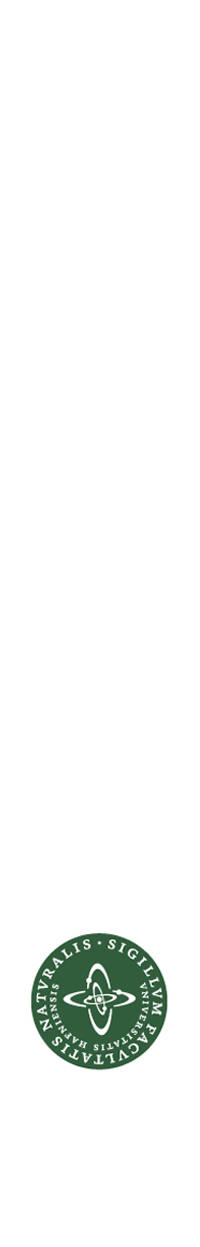
\includegraphics[width=0.15\textwidth]{natlogo.jpg}}

\title{Cryogenic cavity optomechanics with ultrahigh-Q membrane resonators}
\subtitle{Supervisor: Eugene Polzik}
\author{Willi Carlsen}
\institute{Quantop \\Niels Bohr Institute \\University of Copenhagen}
\date{September 2015}
\begin{document}


\frame{\titlepage\vspace{-0.5cm}}

\section{Key points}

\frame{
\frametitle{Key points}
\begin{enumerate}
	\item{Introduction to cavity optomechanics}
	\item{Membrane resonator}
	\item{Optical resonator}
	\item{Questions?}
\end{enumerate}
}


\section{Introduction}

\frame{
\frametitle{Introduction to cavity optomechanics}

}

\section{Membrane}
\frame{
\frametitle{Membrane sample}
\begin{columns}
\begin{column}{0.45\textwidth}
\begin{itemize}
\item Silicon frame
\item Silicon nitride membrane
\item Phononic bandgap shielding bridge
\end{itemize}
\end{column}
\begin{column}{0.45\textwidth}
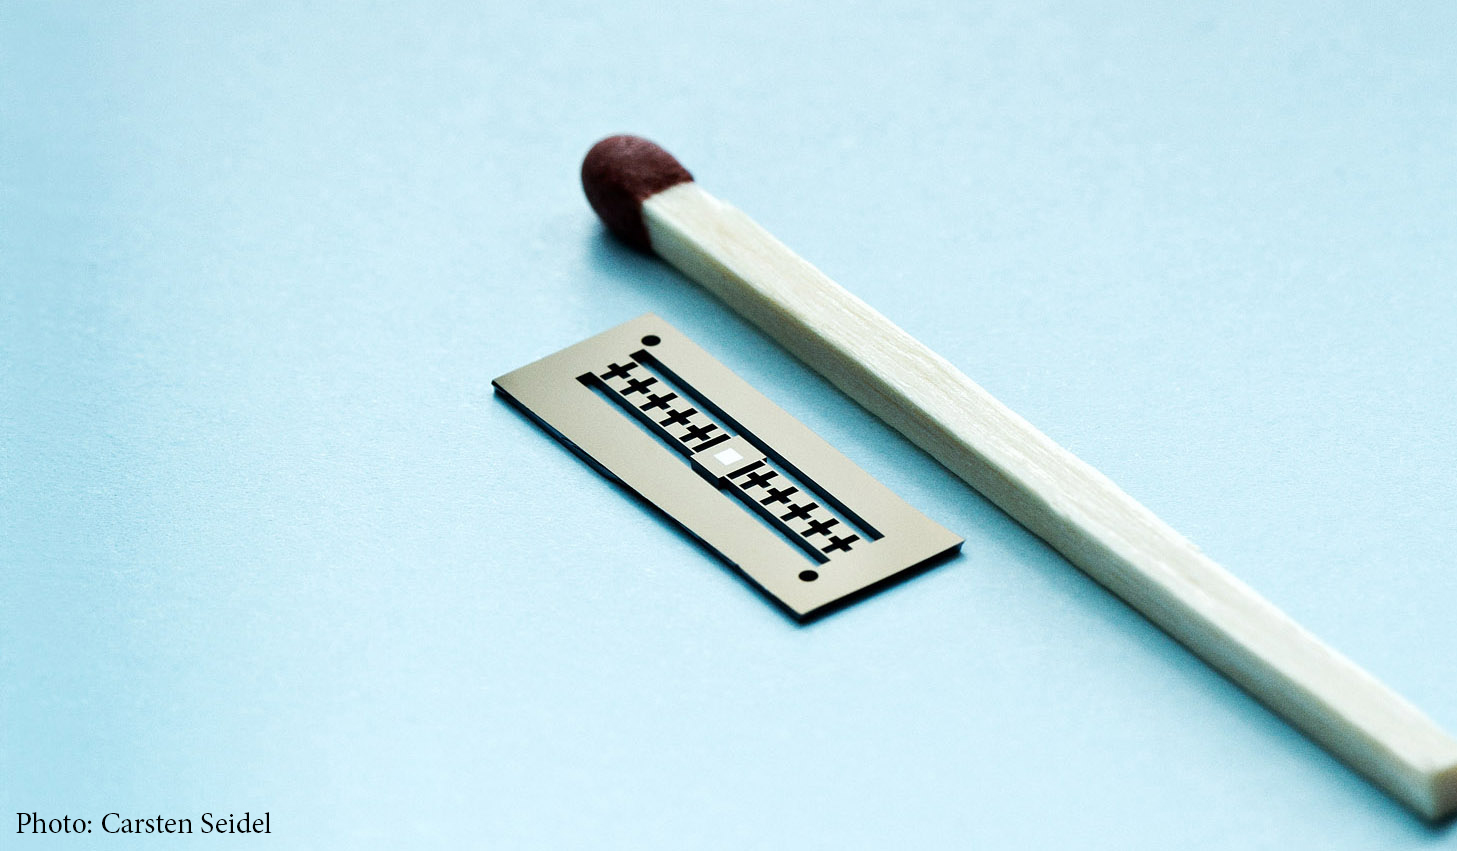
\includegraphics[scale=0.14]{Seidel_02.jpg}
\end{column}
\end{columns}
}

\frame{
\frametitle{Vibrational modes}
\begin{columns}
\begin{column}{0.40\textwidth}
\begin{itemize}
\item Multiple vibrational modes
\end{itemize}
$\Omega_{m,n} = \frac{\pi}{l}\sqrt{\frac{\tau}{\rho}}\sqrt{m^2 + n^2}$\\
\begin{itemize}
\item Effective mass
\end{itemize}
$m_{eff} = \frac{m}{4}$
\end{column}
\begin{column}{0.5\textwidth}
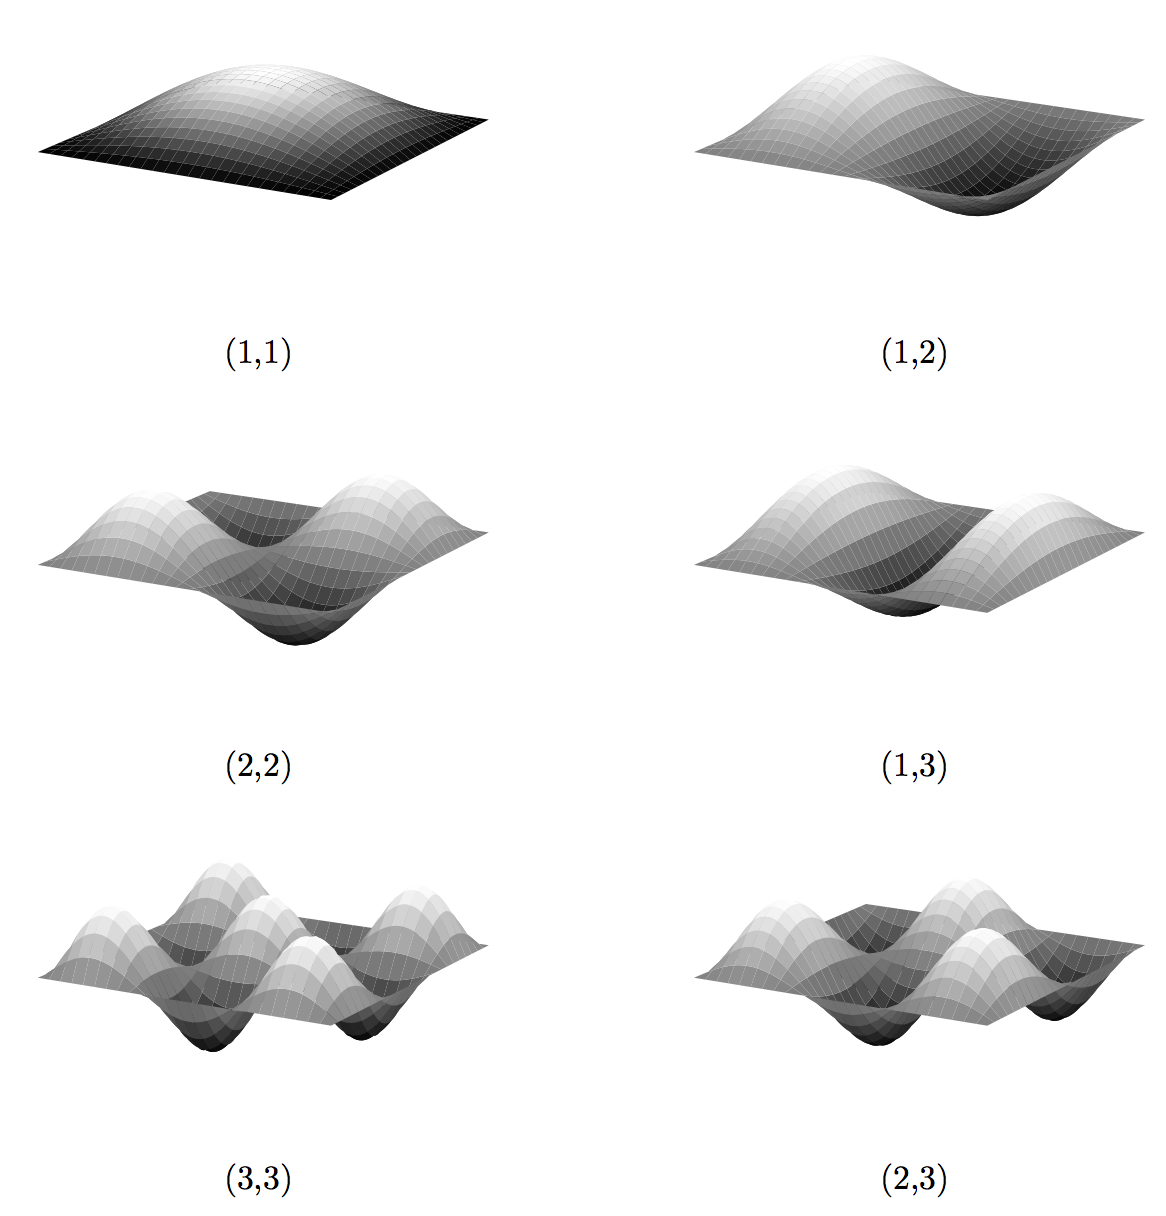
\includegraphics[scale=0.3]{modes.png}
\end{column}
\end{columns}
}

\frame{
\frametitle{Membrane resonator}
\begin{itemize}
\item Equation of motion (time domain)
\end{itemize}
\begin{equation*}
\left(\ddot{x}(t) + \Gamma_m\dot{x}(t) + \Omega_{m}^2x(t)\right)m = F_{ext}(t)
\end{equation*}
\begin{center}
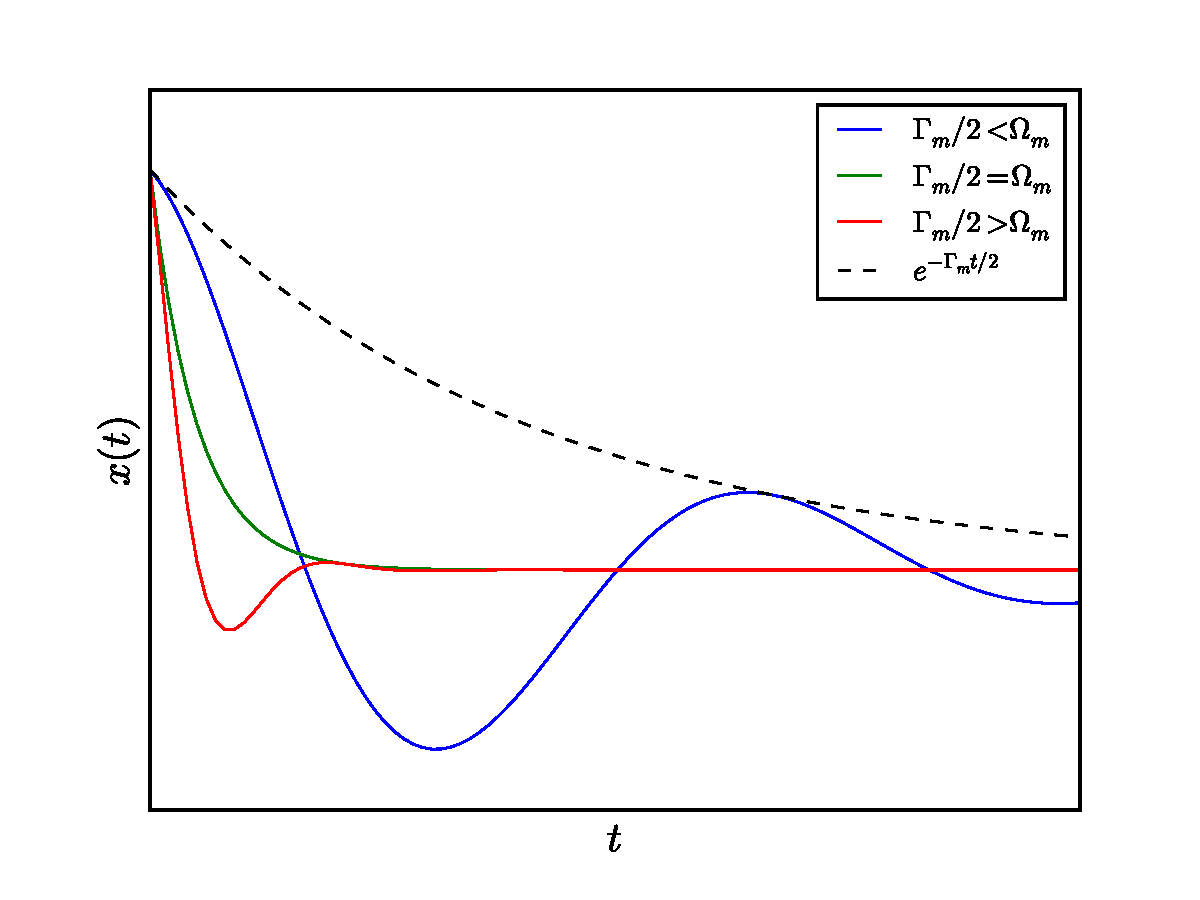
\includegraphics[scale=0.375]{damped_oscillator.pdf}
\end{center}
}

\frame{
\frametitle{Membrane resonator}
\begin{itemize}
\item Quality factor
\end{itemize}
\begin{equation}
Q \equiv \frac{\Omega_m}{\Gamma_m}
\end{equation}
\begin{center}
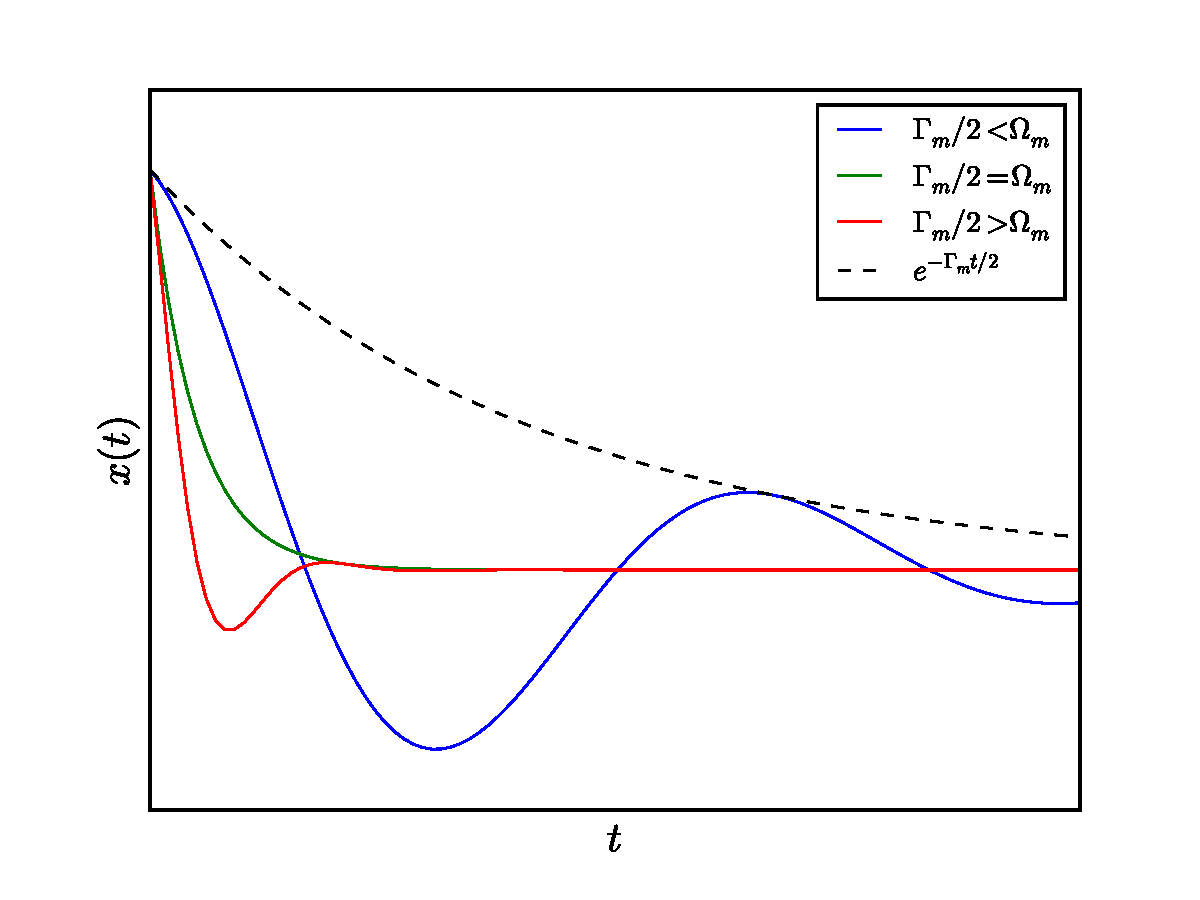
\includegraphics[scale=0.375]{damped_oscillator.pdf}
\end{center}
}

\frame{
\frametitle{Thermal driving force}
What is $F_{ext}$?
\begin{itemize}
\item Membrane couples to the environment ($T_{bath}$)
\item Langevin force $F_{th}$
\end{itemize}
\begin{equation*}
S_{FF}^{th}(\Omega) = \mathcal{F}[\langle F_{th}(t) F_{th}(t + t') \rangle] = 4k_BT_{bath}m_{eff}\Gamma_m
\end{equation*}
}

\frame{
\frametitle{Power spectral density}
\begin{itemize}
\item Power spectral density (frequency domain)
\end{itemize}
\begin{equation*}
S_{xx}(\Omega) = \left|S_{FF}^{th}(\Omega)\chi(\Omega)\right|^2
\end{equation*}
\begin{itemize}
\item Susceptibility
\end{itemize}
\begin{equation*}
 \chi(\Omega)^{-1} = m\left[-\Omega^2 + \Omega_{m}^2 -i\Omega\Gamma_m\right]
\end{equation*}
\begin{itemize}
\item Membrane fluctuations
\end{itemize}
\begin{equation*}
\langle x^2 \rangle = \frac{1}{2\pi}\int_{-\infty}^{\infty}d\Omega S_{xx}(\Omega)
\end{equation*}
}

\frame{
\frametitle{Root mean square displacement}
\begin{itemize}
\item RMS displacement
\end{itemize}
\begin{equation*}
\langle x^2 \rangle = \sqrt{\frac{k_BT_{eff}}{\Omega_{m}^2m_{eff}}}
\end{equation*}
\begin{center}
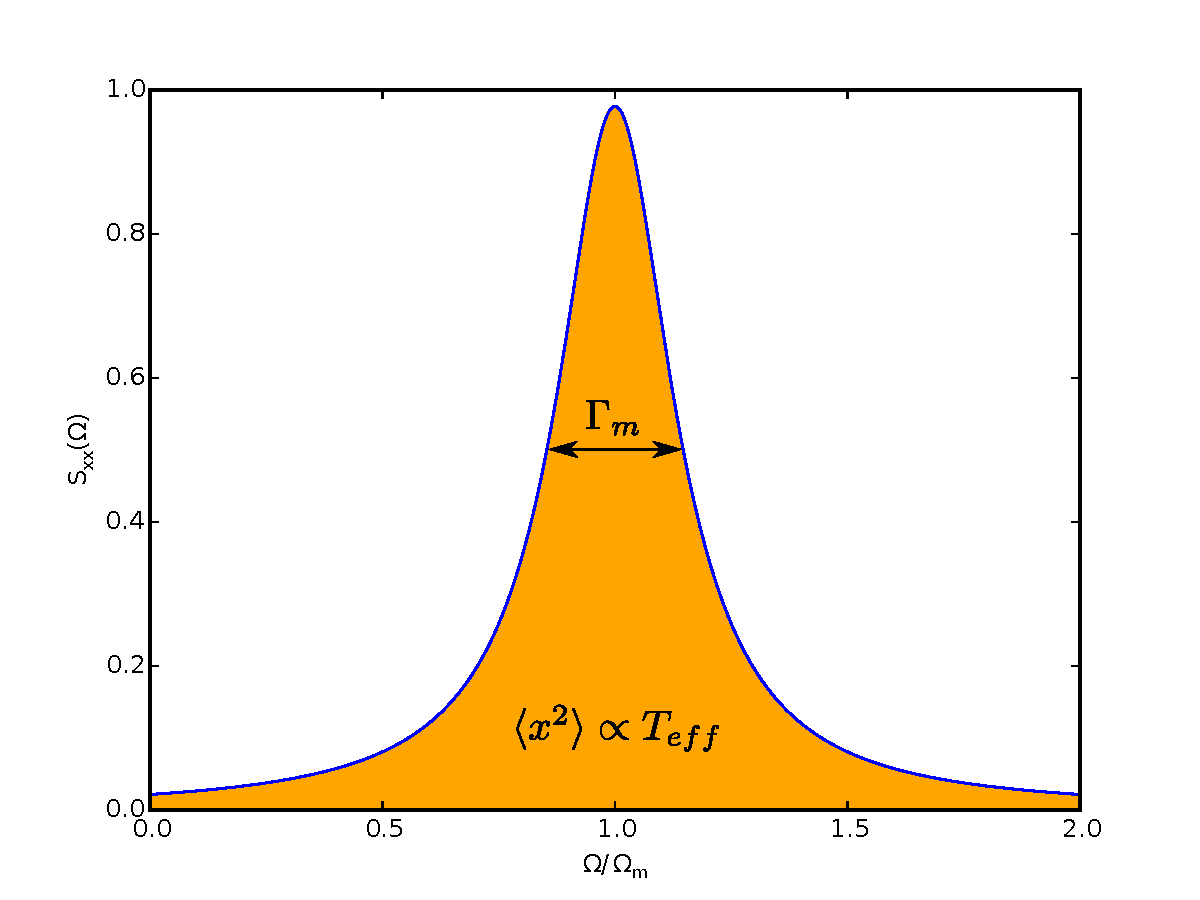
\includegraphics[scale=0.35]{rms.pdf}
\end{center}
}

\frame{
\frametitle{Zero point fluctuation}
\begin{itemize}
\item Quantum mechanical treatment
\end{itemize}
\begin{equation*}
\hat{H}_{mech} = \hbar\Omega_{m}\left(\hat{b}^{\dagger}\hat{b} + \frac{1}{2}\right)
\end{equation*}
\begin{equation*}
\hat{x} = \sqrt{\frac{\hbar}{2m_{eff}\Omega_{m}}}(\hat{b}^{\dagger} + \hat{b})
\end{equation*}
\begin{itemize}
\item RMS displacement
\end{itemize}
\begin{equation*}
\langle \hat{x}^2 \rangle = \frac{\hbar}{2m_{eff}\Omega_{m}}(2\langle\hat{n}\rangle + 1)
\end{equation*}
\begin{itemize}
\item ZPF displacement $\hat{n} = 0$
\end{itemize}
\begin{equation*}
x_{zpf} \equiv \sqrt{\frac{\hbar}{2m_{eff}\Omega_{m}}}
\end{equation*}
}

\frame{
\frametitle{Phononic bandgap}
LOL
}

\section{Cavity}
\frame{
\frametitle{Optical resonator}
\begin{itemize}
\item Fabry-Perot cavity
\end{itemize}
\begin{itemize}
\item Cavity resonances
\end{itemize}
\begin{equation*}
\omega_n = 2\pi\cdot n\frac{c}{2L}
\end{equation*}
\begin{itemize}
\item Free spectral range
\end{itemize}
\begin{equation*}
\omega_{\mathrm{FSR}} = 2\pi\cdot\frac{c}{2L}
\end{equation*}
}

\frame{
\frametitle{Optical resonator}
\begin{itemize}
\item Optical finesse
\end{itemize}
\begin{equation*}
\mathcal{F} = \frac{\omega_{FSR}}{\kappa}
\end{equation*}
\begin{itemize}
\item Loss rates
\end{itemize}
\begin{equation*}
\kappa = \kappa_{ex} + \kappa_{0}
\end{equation*}
}

\frame{
\frametitle{Cavity EOM}
\begin{itemize}
\item Amplitude field analysis
\end{itemize}
\begin{center}
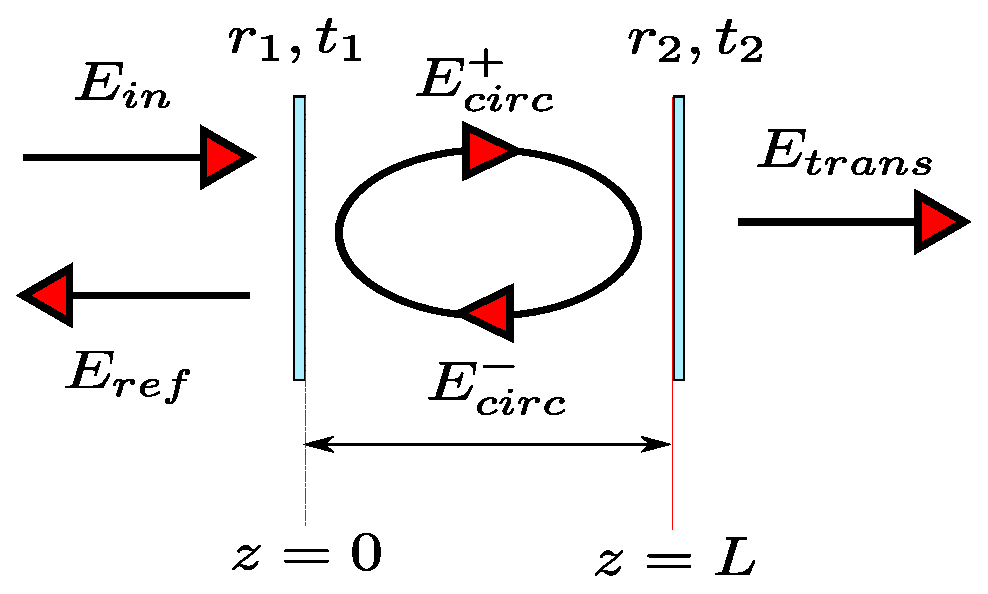
\includegraphics[scale=0.4]{E-field_model_edit.eps}
\end{center}
}

\section{Optomechanics}
\frame{
\frametitle{}

}

\section{Setup}
\frame{
\frametitle{}

}

\section{Experiments}
\frame{
\frametitle{}

}

\section{Conclusion}
\frame{
\frametitle{Conclusion and outlook}
LOL
}


\section{Questions?}

\frame{
\frametitle{Questions?}
\begin{center}
	Questions?
	
	
\includegraphics[scale = 0.500]{questions.jpg}
\end{center}
}

\end{document}